\section{Úvod}
Na konci 19. století se vědci domnívali, že s výjimkou několika detailů jejich teorie dokázaly odpovědět na všechny otázky fyziky. Podle nich už na obzoru nebyly žádné velké objevy. Maxwellovy rovnice elektromagnetismu a Newtonovy pohybové zákony kreslily deterministický vesmír, v němž má každá částice určitou pozici a momentum v daném okamžiku. Síly které působí na částici určují jak se její pozice a rychlost mění v čase.

Ale už v roce 1900, při řešení problému absolutně černého tělesa, objevil Max Planck kvanta. Nedělitelné balíky světla jejichž velikost (energie) závisí na frekvenci daného světla. I když si v té době Max Planck i většina ostatních fyziků myslela, že to je pouze matematický trik, který nemá žádné implikace ve fyzickém světě, byl to první krok vedoucí ke kvantové revoluci.

Albert Einstein věřil ve fyzickou existenci Planckových kvant a ve vlnově-korpuskulární dualitu světla, podle níž je světlo částicí a vlnou zároveň a chová se jako jedno nebo druhé podle způsobu našeho pozorování. Ve svém Annus mirabilis (1905) kvantově vysvětlil fotoefekt: když elektron získá dostatek energie absorbcí kvanta světla, je uvolněn z obalu atomu a následně může být vyzařován.

Francouzský aristokrat Luis de Broglie vzal tento závěr z Planckovy práce ještě dál a teoretizoval o vlnově-korpuskulární dualitě všech částic, nejen světelných, ale také částic hmotných.

Kvantový model atomu se postupně vyvíjel od modelu Nielse Bohra s jedním kvantovým číslem, vyjadřujícím velikost oběžné dráhy elektronu. Arnold Sommerfeld postupně k tomuto modelu přidal 3 další kvantová čísla. Jedno vyjadřující tvar eliptické oběžné dráhy elektronu, druhé (magnetické) vyjadřující orientaci oběžné dráhy v prostoru a poslední vyjadřující spin, což je vnitřní moment hybnosti částice.

V této době bylo zřejmé, že je potřeba vytvořit teorii, která by popisovala fenomény kvantového světa: kvantovou mechaniku.

Roku 1925 Werner Heisenberg přišel na Maticovou kvantovou mechaniku. Maticová, protože ve výpočtech využívá matic a vektorů. Matice jsou tabulky čísel (viz Obrázek \ref{fig:1}, níže), které v této teorii mohou vyjadřovat veličiny jako polohu a hybnost částice. Vektory jsou veličiny které mají kromě velikosti i směr a dají se vyjádřit maticemi. V Maticové mechanice se používají k vyjádření stavu systému. Vzhledem k používaným matematickým prostředkům je tato teorie nesmírně nepraktická k výpočtu vývoje jakéhokoli systému, jelikož rozměry matic se zvyšují exponenciálně s rostoucím počtem částic v systému.

\begin{figure}[ht]
    \centering
    $\begin{pmatrix}
    1 & 0 & 1 \\
    0 & 1 & 0 \\
    1 & 0 & 1
    \end{pmatrix}
    $
    \caption{\label{fig:1}Matice o 3 řádcích a 3 sloupcích.}
\end{figure}

Pouze tři měsíce po vydání Heisenbergova článku o Maticové mechanice zkonstruoval rakouský fyzik Erwin Schrödinger svou proslulou vlnovou rovnici (Rovnice (\ref{eq:1}), níže), která popisuje vývoj vlnové funkce a stala se základem Schrödingerovy vlnové mechaniky. Vlnová mechanika se rychle stala oblíbenější než Maticová, jelikož výpočty s vlnovou rovnicí jsou daleko jednodušší.

\begin{equation}
    i\hbar \frac{\partial \Psi}{\partial t} = -\frac{\hbar^2}{2m}
    \frac{\partial^2 \Psi}{\partial x^2} + V \Psi
    \label{eq:1}
\end{equation}

O rok později Schrödinger dokázal matematickou ekvivalenci Maticové a Vlnové mechaniky. Jsou to dvě formy téže teorie - Kvantové mechaniky.

Ve stejném roce Max Born předložil pravděpodobnostní interpretaci vlnové funkce, ve které, podle Bornova pravidla, druhá mocnina vlnové funkce vyjadřuje pravděpodobnostní distribuční funkci výsledku. Pro ilustraci vezměte v úvahu Obrázek \ref{fig:2}. $\bm{\Psi}$ je vlnová funkce, která vyjadřuje stav systému, např. pozici elektronu. \textbf{P} je pravděpodobnostní distribuční funkce. Tato funkce vyjadřuje pravděpodobnost pro každý možný výsledek měření (každá možná pozice elektronu). $\bm{P(x_0,x_1)}$ je pravděpodobnost, že výsledek měření bude mezi $x_0$ a $x_1$. V našem případě je to pravděpodobnost, že elektron bude mít pozici mezi $x_0$ a $x_1$ a počítá se integrací pravděpodobnost\-ní funkce mezi hodnotami $x_0$ a $x_1$. Integrací $(\int_{x_0}^{x_1}|\Psi|^2\,dx)$ získáme obsah pod křivkou v daném rozsahu, který odpovídá hledané pravděpodobnosti. 




\begin{figure}[ht]
\centering
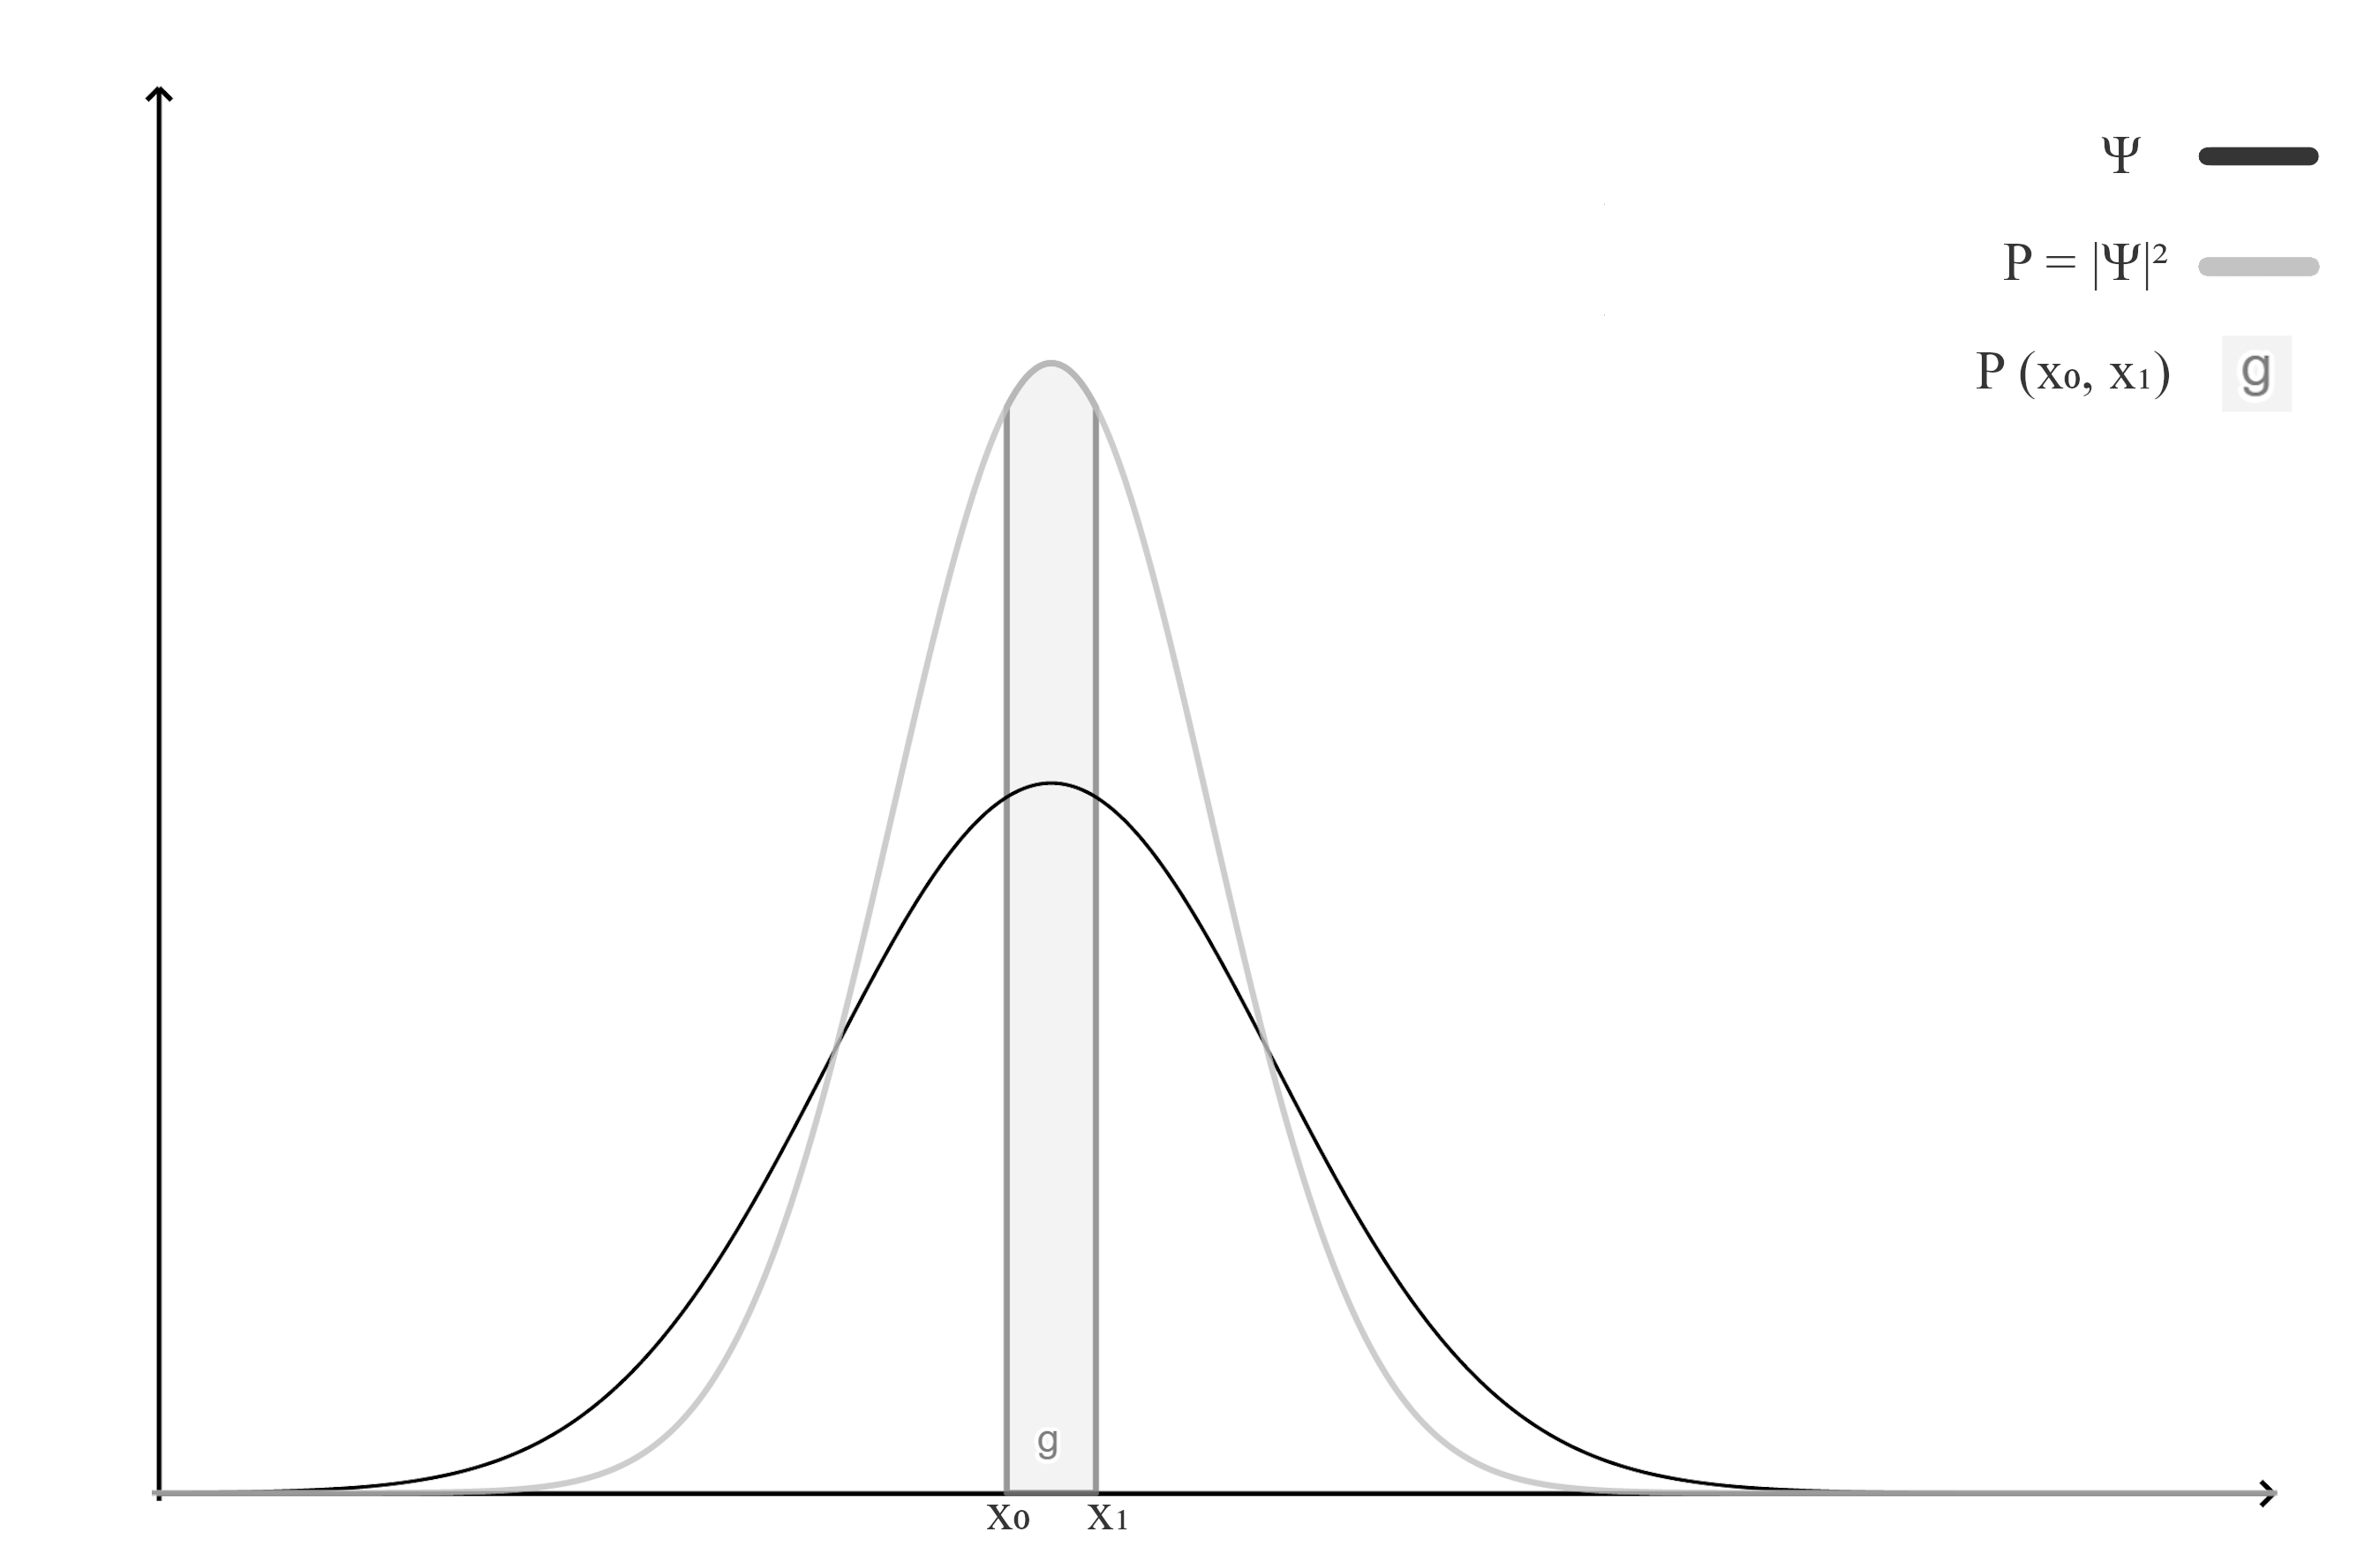
\includegraphics[width=250pt]{images/probability-function.png}
\caption{\label{fig:2}Vlnová funkce, pravděpodobnostní funkce a pravděpodobnost určitého výsledku.}
\end{figure}

Tato pravděpodobnostní interpretace se stala důležitou součástí dnešní Kvantové mechaniky, za kterou je považována Kodaňská interpretace, kterou společně vyhotovili Bohr, Pauli a Heisenberg v Bohrově institutu v Kodani.

Kvantová mechanika změnila obraz vesmíru z deterministického a předurčeného na indeterministický a pravděpodobnostní. V kvantovém pravděpodobnostním vesmíru můžeme určit pouze pravděpodobnost daného výsledku. Jediný způsob jak Clerk Maxwell a Ludwig Boltzmann mohli popsat vlastnosti plynu, skládajícího se z nesčetného množství částic bylo použitím pravděpodob\-nosti a museli se spokojit se statistickým popisem. Tento nucený ústup ke statistické analýze byl způsoben neuskutečnitelností sledování pozice a rychlosti tolika částic. Pravděpodob\-nost byla důsledkem lidské ignorance. Naopak podle Kvantové mechaniky toto pravděpodobnost\-ní vyjádření kvantového světa není způsobeno lidskou nevědomostí, ale je fundamentální vlastností kvantového vesmíru.

Přes jeho účast v začátcích kvantové revoluce se Albert Einstein stal jejím největším kritikem. Uvědomoval si její užitečnost v atomových měřítcích, ale myslel si, že \uv{Bůh ne{hraje v }kostky.} Byl přesvědčený, že kvantová mechanika není konečnou teoríí, že za ní musí být fundamentálnější deterministická teorie. Takovým teoriím se říká teorie se \uv{skrytými} parametry. Podle těchto teorií dokážeme určit jen pravděpodobnost výsledků, jelikož neznáme všechny parametry. Kdybychom znali tyto \uv{skryté} parametry, dokázali bychom určit přesný výsledek měření.

V roce 1962 našel John Stewart Bell způsob jak matematicky posoudit možnost teorie se skrytými parametry, která by replikovala výsledky kvantové mechaniky. Dnes se jí říká Bellova nerovnost. Tato nerovnost byla experimentálně porušena. Podle všeobecného mínění znamená porušení této nerovnosti nemožnost teorie se skrytými parametry. Toto porušení ale pouze znamená, že neexistuje teorie se skrytými parametry, která splňuje princip lokality a podmínku statistické nezávislosti.

V této práci se budu věnovat teorii se skrytými parametry, která nesplňuje podmínku statistické nezávislosti. Takovou teorii nazval Bell Superdeterminismus. Statistická nezávislost (viz Rovnice (\ref{eq:2}), níže) znamená, že pravděpodobnostní distribuce skrytých parametrů, $\bm{p(\lambda)}$, se nezmění když vezmeme v potaz nastavení detektorů, \textbf{(a,b)}. Této podmínce se často říká podmín\-ka svobodné vůle, nebo svobodné volby. 

Cílem této práce je přehodnocení argumentů proti Superdeterminismu. Pokusím se vysvětlit, v rozporu s všeobecným míněním, že Superdeterminismus je cestou, která by mohla vyřešit mnoho problémů se současnými teoriemi, a kterou bychom neměli ignorovat; je to cesta kterou jsme se nevydali.

\begin{equation}
    p(\lambda|\bm{a},\bm{b}) = p(\lambda) 
    \label{eq:2}
\end{equation}

